
% Chapter 2

\chapter{Nuclear Matter: Hot and Cold} % Main chapter title
%----------------------------------------------------------------------------------------
\section{Hot versus Cold Nuclear Matter}
Because the deconfinement corresponds to a condition where the temperature of the system is above some critical temperature it is often called "Hot Nuclear Matter." Therefore, the region of the nuclear matter phase diagram where quarks and gluons are confined to baryon and meson states is often called "Cold Nuclear Matter." Historically, "Hot" QGP systems were those created by colliding two large nuclei such as in Au+Au collisions and "Cold Nuclear Matter" systems were made by colliding large nuclei with smaller ones such as in d+Au collisions and in beam collisions with fixed nuclear targets. 

\section{The Cronin Effect}
The seminal paper titled \textbf{Production of hadrons at large transverse momentum at 200, 300, and 400 GeV} by J.W. Cronin, et al. detailed a fixed target experiment that collided protons with a tungsten target and underpinned a phenomenon found in cold nuclear matter systems. Later dubbed the \textit{Cronin Effect} after the paper's first author, the experiment found that the production of protons at mid $p_{T}$ ($2\leq p_{T} \leq 4$) was enhanced when compared to the production of pions \citep{croninpaper}. 
\begin{figure}[htbp!]
  \centering
    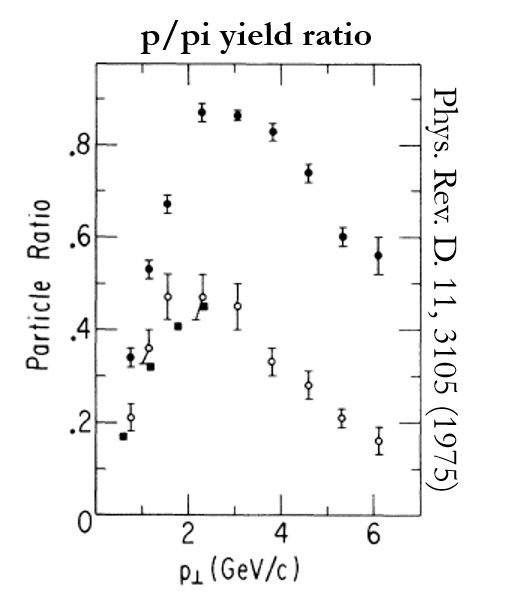
\includegraphics[width=0.5\textwidth]{prevplots/croninratio.JPG}
    \rule{35em}{0.5pt}
  \caption[Proton vs pion yield ratio from the Cronin paper]{Proton vs pion yield ratio from the Cronin paper. Closed circles are the ratio obtained by colliding 23.7 $GeV/c^{2}$ protons on tungsten (A=110). Open circles are the same data extrapolated (A=1).}
  \label{fig:croninratio}
\end{figure}

After this discovery many set out to come up with theoretical mechanisms that could explain this baryon production preference. These mechanisms can largely be categorized into two types: those where the incoming partons interact with the nuclear medium and those where outgoing partons created after an incoming nucleon hard scatters interacts with the nuclear medium. These two categories are called \textit{Initial State Interactions} and \textit{Final State Interactions.}

\subsection{Initial State Multiple Scattering}
The first attempts at explaining the Cronin Effect were made using initial state interactions. Kühn in 1975 described a mechanism where incoming quarks scatter with nuclear quarks which randomize the direction of the incoming parton before finally colliding with another quark to produce an event similar to a proton-proton collision\citep{PhysRevD.13.2948}. Since it is unclear how many "soft scatters" happen before the final hard scatter the $p_{T}$ spectrum is broadened which could account for the increase of particle production for the mid $p_{T}$ range. 
\begin{figure}[htbp!]
  \centering
    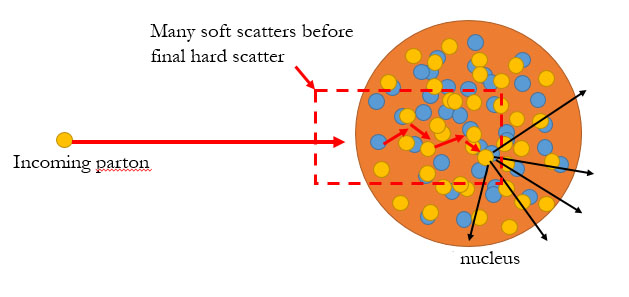
\includegraphics[width=0.8\textwidth]{Figures/ISIscattering.jpg}
    \rule{35em}{0.5pt}
  \caption[Illustration of Initial State Multiple Scattering]{Illustration of Initial State Multiple Scattering.}
  \label{fig:ISIscattering}
\end{figure} 

The NA10 collaboration at CERN set out to use back to back lepton probes to study the effect of the nucleus on jets. They collided 140 GeV and 258 GeV negative pions on tungsten targets of various thicknesses and looked for muon pairs produced via a Drell-Yan Process. 

\begin{figure}[htbp!]
  \centering
    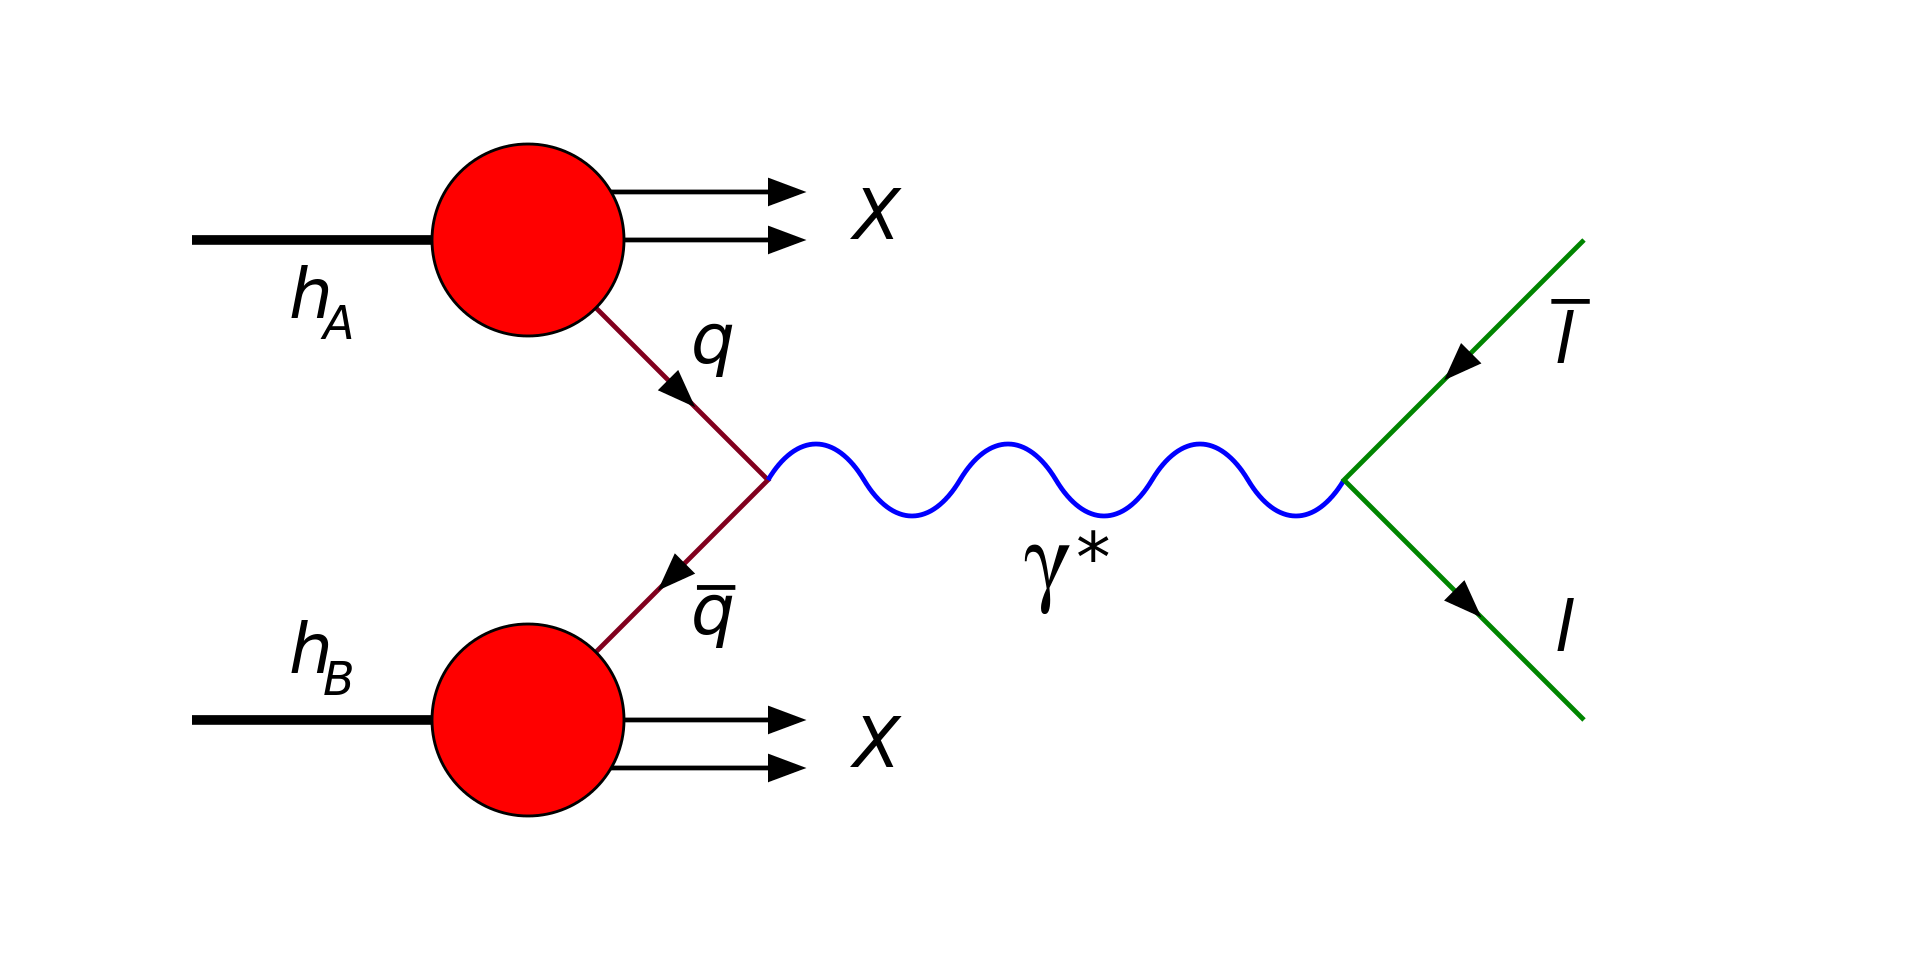
\includegraphics[width=0.7\textwidth]{Figures/DYfeynman.png}
    \rule{35em}{0.5pt}
  \caption[Feynman diagram of Drell-Yan production of dileptons.]{Feynman diagram of Drell-Yan production of dileptons. Quark-Antiquark annihilation produces a lepton-antilepton pair through the exchange of a virtual photon.\citep{PhysRevLett.25.316}}
  \label{fig:DYfeynman}
\end{figure}

They found that the mean squared $p_{T}$ did not vary much at all as a function of target thickness which implies that incident partons are not affected by the thickness of the target and therefore that the path length of soft collisions that would broaden the $p_{T}$ spectrum is very short. Furthermore, the E772 collaboration, with an experiment colliding 800 GeV protons on H$_{2}$, C, Ca, Fe, and W targets, showed that Drell-Yan produced dileptons’ mean squared $p_{T}$ did not vary much between the nuclear targets of varying nucleon number.\citep{PhysRevLett.66.2285} i.e. increasing the number of nucleons does not change the net $p_{T}$ much, further showing that initial state contributions to $p_{T}$ broadening is minimal.

\subsection{Final State Multiple Scattering}
In 1991 the E609 collaboration at Fermilab studied dijets produced in fixed target experiments colliding 400 $GeV/c$ protons with targets made of various nuclear materials including hydrogen and lead\citep{Corcoran:1990vq}. The conditions of interest to them were the creation of two back to back jets produced after an incoming parton hard scattered with a target nucleon. 
They defined a quantity called \textit{planarity} which measured how \textit{back-to-back} two jets are. In their words:
\begin{addmargin}[1.5em]{2em}
"An axis is found which maximizes the sum of the squares of all momentum components ($b_{max}$) along that axis while minimizing the sum of the squares of momentum components perpendicular to that axis ($b_{min}$). Planarity is then defined as: 
\begin{equation}
P = \frac{b_{max}-b_{min}}{b_{max}+b_{min}}.
\end{equation}
For two narrow back-to-back jets P approaches 1, while for a circularly symmetric event P is 0."
\end{addmargin}

\begin{figure}[htbp!]
  \centering
    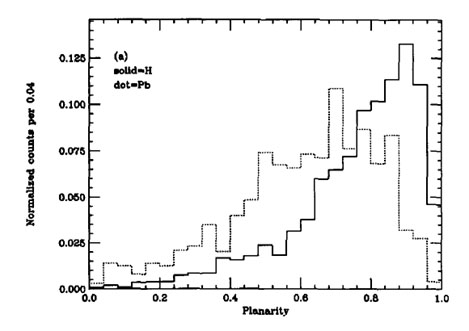
\includegraphics[width=0.8\textwidth]{prevplots/e609planarity.jpg}
    \rule{35em}{0.5pt}
  \caption[Planarity of jets created with protons incident on Pb targets vs H targets.]{Planarity of jets created with protons incident on Pb targets vs H targets.}
  \label{fig:e609planarity}
\end{figure}
Their measurement compared the planarity of dijets created from protons colliding with a hydrogen target with the planarity of those created with collisions on a lead target. They noticed a downward shift in planarity and broadening of the spectrum for Pb dijets compared to H although both had very similar jet widths. This measurement led to a paper in 1993 where they concluded that “Parton hard scatterings within nuclei involve very little nuclear scattering of the incident parton, but that there is substantial nuclear rescattering of outgoing hard scattered partons.\citep{PhysRevLett.70.143}” Because of this, we call this type of mechanism a \textit{Final State Interaction}. While it is true that this could account for the increase in particle production it does not effectively explain why the effect is stronger for baryons than for mesons and why this preference disappears for at high $p_{T}$
\begin{figure}[htbp!]
  \centering
    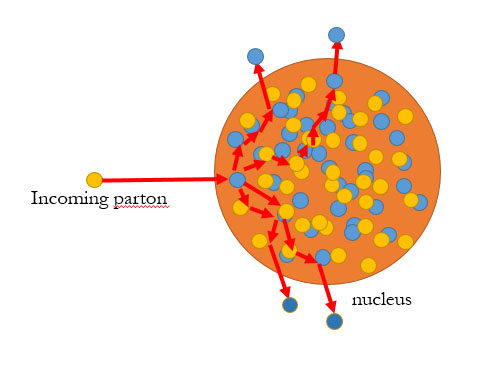
\includegraphics[width=0.7\textwidth]{Figures/FSIscattering.jpg}
    \rule{35em}{0.5pt}
  \caption[Illustration of Final State Multiple Scattering]{Illustration of Final State Multiple Scattering.}
  \label{fig:FSIscattering}
\end{figure} 

\section{Hot Nuclear Matter: QGP}
So far this discussion has stayed within the temperature regime where quarks and gluons are confined to hadronic states. As summarized in the previous chapter, physicists had already seen enough hints that new physics was taking place when the energy density reached some critical value and consequently RHIC was commissioned to study this phase change.

\subsection{Baryon Enhancement}

\begin{figure}
\centering
\begin{subfigure}[b]{0.7\textwidth}
    \centering
    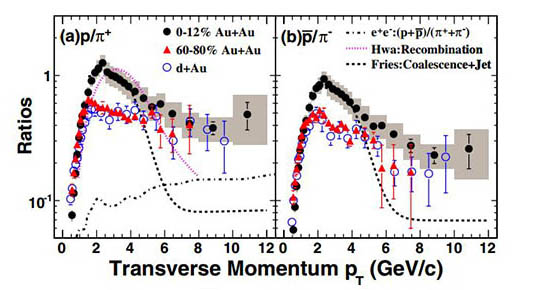
\includegraphics[width=\textwidth]{prevplots/ppiratiocentvsperiph.JPG}
    \caption{ $p/\pi{+}$ and $\bar{p}/\pi^{-}$ ratios for central and peripheral 200 GeV Au+Au collisions. Two leading models are compared to the data as well as the same ratio for 200 GeV d+Au collisions.}
    \label{fig:ppiratiocentvsperiph}
\end{subfigure}
\begin{subfigure}[b]{0.8\textwidth}
    \centering
    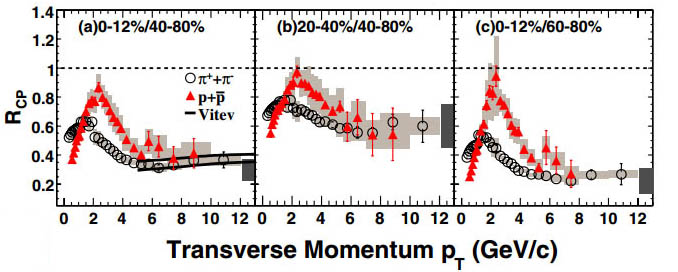
\includegraphics[width=\textwidth]{prevplots/Rcpcentvsperiph.jpg}
    \caption{Nuclear modification factor, $R_{CP}$, comparing nuclear effects on particle production in central versus peripheral Au+Au collisions compared to production in binary scaled p+p collisions}
    \label{fig:Rcpcentvsperiph}
\end{subfigure}
\caption[Evidence of Baryon Enhancement in Au+Au collisions]{$p/\pi$ production ratio and $R_{CP}$ as evidence of Baryon Enhancement in central Au+Au}
\label{fig:baryonenhancementAA}
\end{figure}

One of the surprises encountered when studying this new phase of matter was that the production of particles seemed to have a different mechanism compared to p+p collisions. One experimental signature of this was the so called \textit{baryon enhancement} for peripheral Au+Au collisions \citep{PhysRevLett.97.152301}. This result is shown in figure \ref{fig:ppiratiocentvsperiph} which shows the comparative yield between protons and pions in bins of $p_{T}$. The phenomena of interest is the apparent baryon excess in central collision data set for the mid $p_{T}$ range which is strongest at around $p_{T}\approx$ 2 GeV/c and disappears at around $p_{T}\approx$ 4 GeV/c. Similarly, the Nuclear Modification factor for Central and Peripheral collisions also shows this enhancement in the same range (shown in figure \ref{fig:Rcpcentvsperiph}).

\subsection{Theoretical Models of Baryon Enhancement}
Though many have proposed models to describe this baryon enhancement, I will focus this discussion on the two leading models.

\subsubsection{Recombination}
Following the idea that a phase change in nuclear matter happens when a critical energy density causes deconfinement of quarks and gluons from their bound states as neutrons and protons and that the post-collision evolutionary behavior of this QGP is one that expands rapidly, Rudolph Hwa and C.B. Yang postulated that the enhancement of particle production could be explained by the ways in which the outgoing partons interacted\citep{PhysRevC.70.024905}. They defined two types of partons, those with low transverse momentum created by the hydrodynamic outward expansion of the QGP referred to as \textit{soft} and/or \textit{thermal} partons and those with high transverse momentum created by \textit{hard} nuclear scattering processes or \textit{shower} partons. The production of particles could then be described by the way these partons combined combinatorically, i.e. the way thermal partons combined with other thermal partons, the way they combined with shower partons, and the way shower partons combined with other shower partons. This mechanism was termed \textit{recombination} since it relied on the recombining of quarks in partons created from the nuclear collision.

\begin{figure}
\centering
\begin{subfigure}[b]{0.32\textwidth}
    \centering
    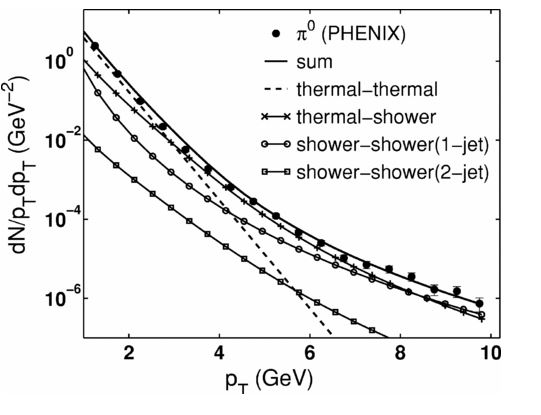
\includegraphics[width=\textwidth]{prevplots/piyieldrecomb.JPG}
    \caption{$p_T$ distribution of pions}
    \label{fig:kyieldrecomb}
\end{subfigure}
\begin{subfigure}[b]{0.32\textwidth}
    \centering
    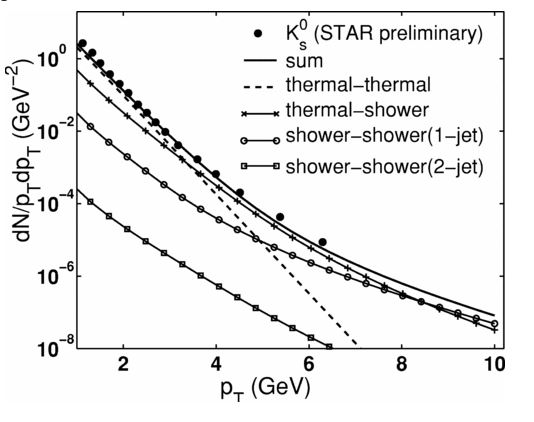
\includegraphics[width=\textwidth]{prevplots/kyieldrecomb.JPG}
    \caption{$p_T$ distribution of kaons}
    \label{fig:kyieldrecomb}
\end{subfigure}
\begin{subfigure}[b]{0.32\textwidth}
    \centering
    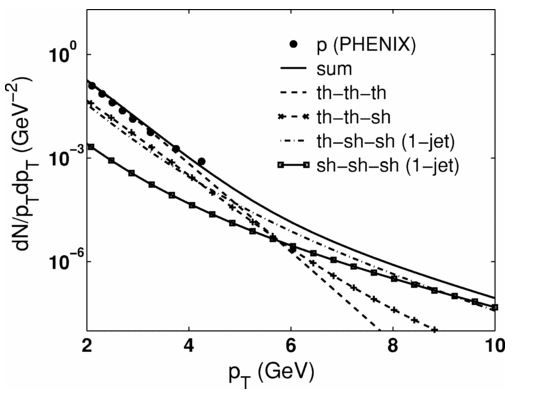
\includegraphics[width=\textwidth]{prevplots/pyieldrecomb.JPG}
    \caption{$p_T$ distribution of protons}
    \label{fig:pyieldrecomb}
\end{subfigure}
\begin{subfigure}[b]{0.5\textwidth}
    \centering
    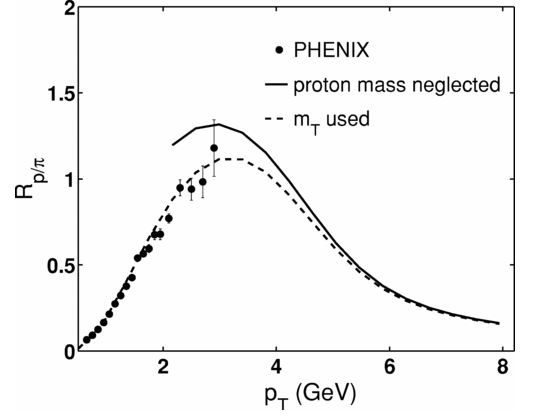
\includegraphics[width=\textwidth]{prevplots/ppiratiorecomb.JPG}
    \caption{$p/\pi$ production ratio versus $p_T$}
    \label{fig:ppiratiorecomb}
\end{subfigure}
\caption[Recombination model compared with Au+Au data]{Au+Au identified particle measurements compared with recombination model predictions. For the $p_T$ distributions we see three distinct regions of recombination, the low $p_T$ range where soft thermal parton recombination dominates, the high $p_T$ range where hard shower parton recombination dominates, and the middle range where thermal-shower recombination best describes the data.}
\label{fig:hwaAAmodels}
\end{figure}

\subsubsection{Fragmentation}
\begin{figure}[htbp!]
  \centering
    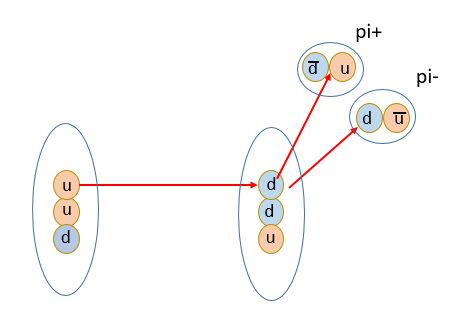
\includegraphics[width=0.5\textwidth]{Figures/fragmentationdiag.JPG}
    \rule{35em}{0.5pt}
  \caption[Illustration of an example hard scatter resulting in fragmentation to two pions]{Illustration of an example hard scatter resulting in fragmentation to two pions. Here an up quark scatters with enough energy to scatter and release the down quark from being bound in another nucleon. This occurs with enough energy to create antiparticle partners from the vacuum resulting in the formation of charged pions.}
  \label{fig:fragmentationdiag}
\end{figure} 
Fries, M{\"u}eller, Nonaka, and Bass postulated that the the reason why protons were produced in abundance was simply that following a collision, the building blocks of protons: up and down quarks, are plentiful and that they simply recombine back into their confined states. This mechanism dominates for low $p_{T}$ since outgoing partons are traveling slowly which allows the constituent quarks to remain connected by a color string. In contrast to the soft thermal partons, partons created with hard scattering processes are more likely to break the color string creating quark/anti-quark pairs, i.e. mesons. Because this range of $p_{T}$ causes individual quarks in the QGP to fragment out, the lone quarks scatter off with enough energy to create quark antiquark pairs from the vacuum which pair up with the nuclear quarks . This two regime model naturally creates a baryon preference for low $p_{T}$ partons that is met with proportional meson production when the parton $p_{T}$ is adequately high enough.

\section{Flow at the LHC}
Up till now it appeared that the lines in the proverbial sand were clear with respect to nuclear matter phase changing and that we had two distinct ways to measure the properties of these two states. There is cold hadronic matter which has its own experimental signatures that are measured with beam on fixed target experiments and with small ion (protons and deuterons) on heavy ion collisions and hot deconfined quark matter which flows and behaves another way and studied using collisions of two heavy nuclei. This notion that the two experimental methods allowed the temperature dependent phenomena to be studied separately was brought into question in 2015 when the Large Hadron Collider (LHC) at CERN turned on and entered its second era of measurements. At the Compact Muon Solenoid (CMS) they collected data from p+Pb collisions at 5.02 TeV and compared it to Pb+Pb collisions at 2.76 TeV. While hydrodynamic phenomena like collective flow was expected in the Pb+Pb data, they found the unexpected when a nonzero elliptic flow was measured in p+Pb (see fig \ref{fig:pPbflow}).
\begin{figure}[htbp!]
  \centering
    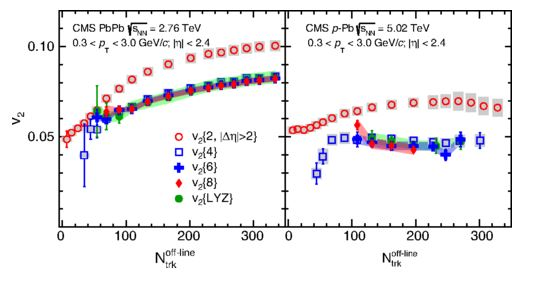
\includegraphics[width=0.7\textwidth]{prevplots/pPbflowLHC.JPG}
    \rule{35em}{0.5pt}
  \caption[Elliptic Flow in p+Pb at the LHC]{CMS result from 5.02 TeV p+Pb collisions showing a nonzero elliptic flow signal versus track multiplicity}
  \label{fig:pPbflow}
\end{figure} 

The appearance of flow in systems previously thought of as "cold" was a sign that perhaps the QGP forms much easier than previously expected and that perhaps some phenomena found in cold systems, such as baryon enhancement, could be attributed to mechanisms that found favor in explaining similar phenomena in hot heavy ion systems.

\section{Recombination and Fragmentation for All?}
Furthermore, experimental evidence that the two systems behave quite similarly has been found. In fig. \ref{fig:daaaratios} particle production ratios ($p/\pi$) are compared and we see that the baryon enhancement which was indicative of the QGP formation in peripheral Au+Au collisions is followed extremely closely by data from central d+Au. 

\begin{figure}[htbp!]
  \centering
    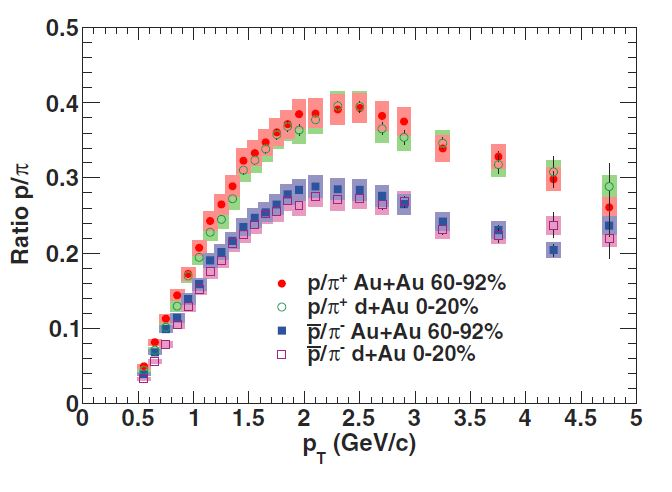
\includegraphics[width=0.7\textwidth]{prevplots/dAvsAAratios.JPG}
    \rule{35em}{0.5pt}
  \caption[p/$\pi$ ratios compared for central d+Au and peripheral Au+Au]{p/$\pi$ ratios compared for central d+Au and peripheral Au+Au\citep{PhysRevC.88.024906}}
  \label{fig:daaaratios}
\end{figure} 

It may seem that the behavior of the two are contradicting since one is central and the other peripheral but we can see that the geometries of the collisions for the two cases are similar. The glancing peripheral Au+Au collisions create an "almond-like" QGP fireball whereas peripheral collisions in d+Au would behave such as a p+p collision since the number of participants is at a minimum when the collision is maximally peripheral. If we make the hypothesis that QGP formation is most likely with a higher number of participants then it follows that central d+Au collisions would be most likely to form a QGP. And so since physicists love reductionism and unification, and that the evidence makes one wonder if a QGP is formed in simpler systems, it would be advantageous to be able to describe the two systems with a singular mechanism.

But are there even the building blocks to support such a notion that QGP is created in such a simple system as d+Au? Recombination is easy to justify in Au+Au since the large number of participants makes the formation of the QGP easily achieved and leaves a great abundance of free quarks that are able to recombine. What if we apply the same ideas to d+Au? 
\begin{figure}[b!]
  \centering
    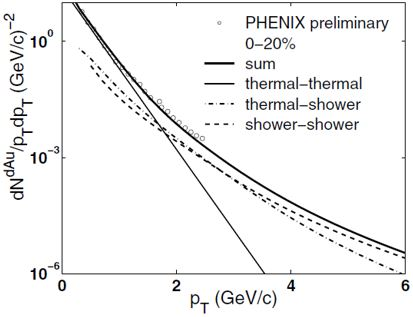
\includegraphics[width=0.5\textwidth]{prevplots/daurecomb.JPG}
    \rule{35em}{0.5pt}
  \caption[Pion transverse momentum distribution from d+Au collisions compared to one created with the recombination model]{Pion transverse momentum distribution from d+Au collisions compared to one created with the recombination model}
  \label{fig:daaaratios}
\end{figure}
Hwa and Yang asserted \citep{PhysRevLett.93.082302} that since hard scattering creates jets, jet formation generates a lot of soft outgoing partons. Furthermore, soft partons behave like an expanding QGP, that is to say, they behave like thermal partons. Thermal parton baryon enhancement is due to recombination. Since soft partons behave like thermal partons, could there recombination in d+Au, and if there is, could it be a sign that we should see other signs of QGP formation such as collective flow? 

I postulate that there is sufficient evidence to say that the nuclear matter created by d+Au behaves collectively and that there should be a non-zero elliptic flow measurement. Furthermore, this elliptic flow is dependent on particle species in that it exhibits baryon enhancement in the mid $p_T$ range indicative of the formation of a QGP. Unknown phenomena of interest is the enhancement of strangeness. Recall that early fixed target experiments exhibited enhanced production of kaons compared to binary collisions, however there is no such enhancement in Au+Au collisions. Evidence of kaon flow or lack thereof could point to an interesting difference in the physics of the two different systems.

\pagebreak
\pagebreak
